\section{Testing}
\subsection{Gate driver}\label{Gate driver}
In the initial phase of testing, the focus was on evaluating the gate drivers. Extensive testing and measurements were conducted. Initially, the IRS2004SPBF\cite{infineon-irs2004-datasheet} was utilized due to the sinusoidal signal being sent from the STM32F411\cite{stm32-base-board} to the gate drivers. However, both the code and hardware lacked optimization, leading to rapid heating of the BLDC motor\cite{reichelt-motor-datasheet} and increased current consumption(3+ amps) even under no load conditions, as illustrated in \autoref{fig:BLDCHEAT}. Subsequently, a shift in approach was made, opting for a block signal with the IRS2001SPBF\cite{infineon-irs2001-datasheet} gate driver. Although improved results were observed, the motor still exhibited some warmth, albeit less pronounced. To delve deeper into signal processing, the decision was made to alter the bootstrap resistors from 5 ohms to 1 ohm, effectively mitigating the occurrence of a small short (\autoref{fig:smallshort}). This adjustment proved to be pivotal. As a result, the BLDC motor\cite{reichelt-motor-datasheet} can now operate for 5 minutes at 4800 RPM without exceeding 50 degrees Celsius and staying below 250 mA, marking a significant achievement.
\begin{figure}[H]
    \centering
    \hfill
    \begin{subfigure}{0.42\textwidth}
        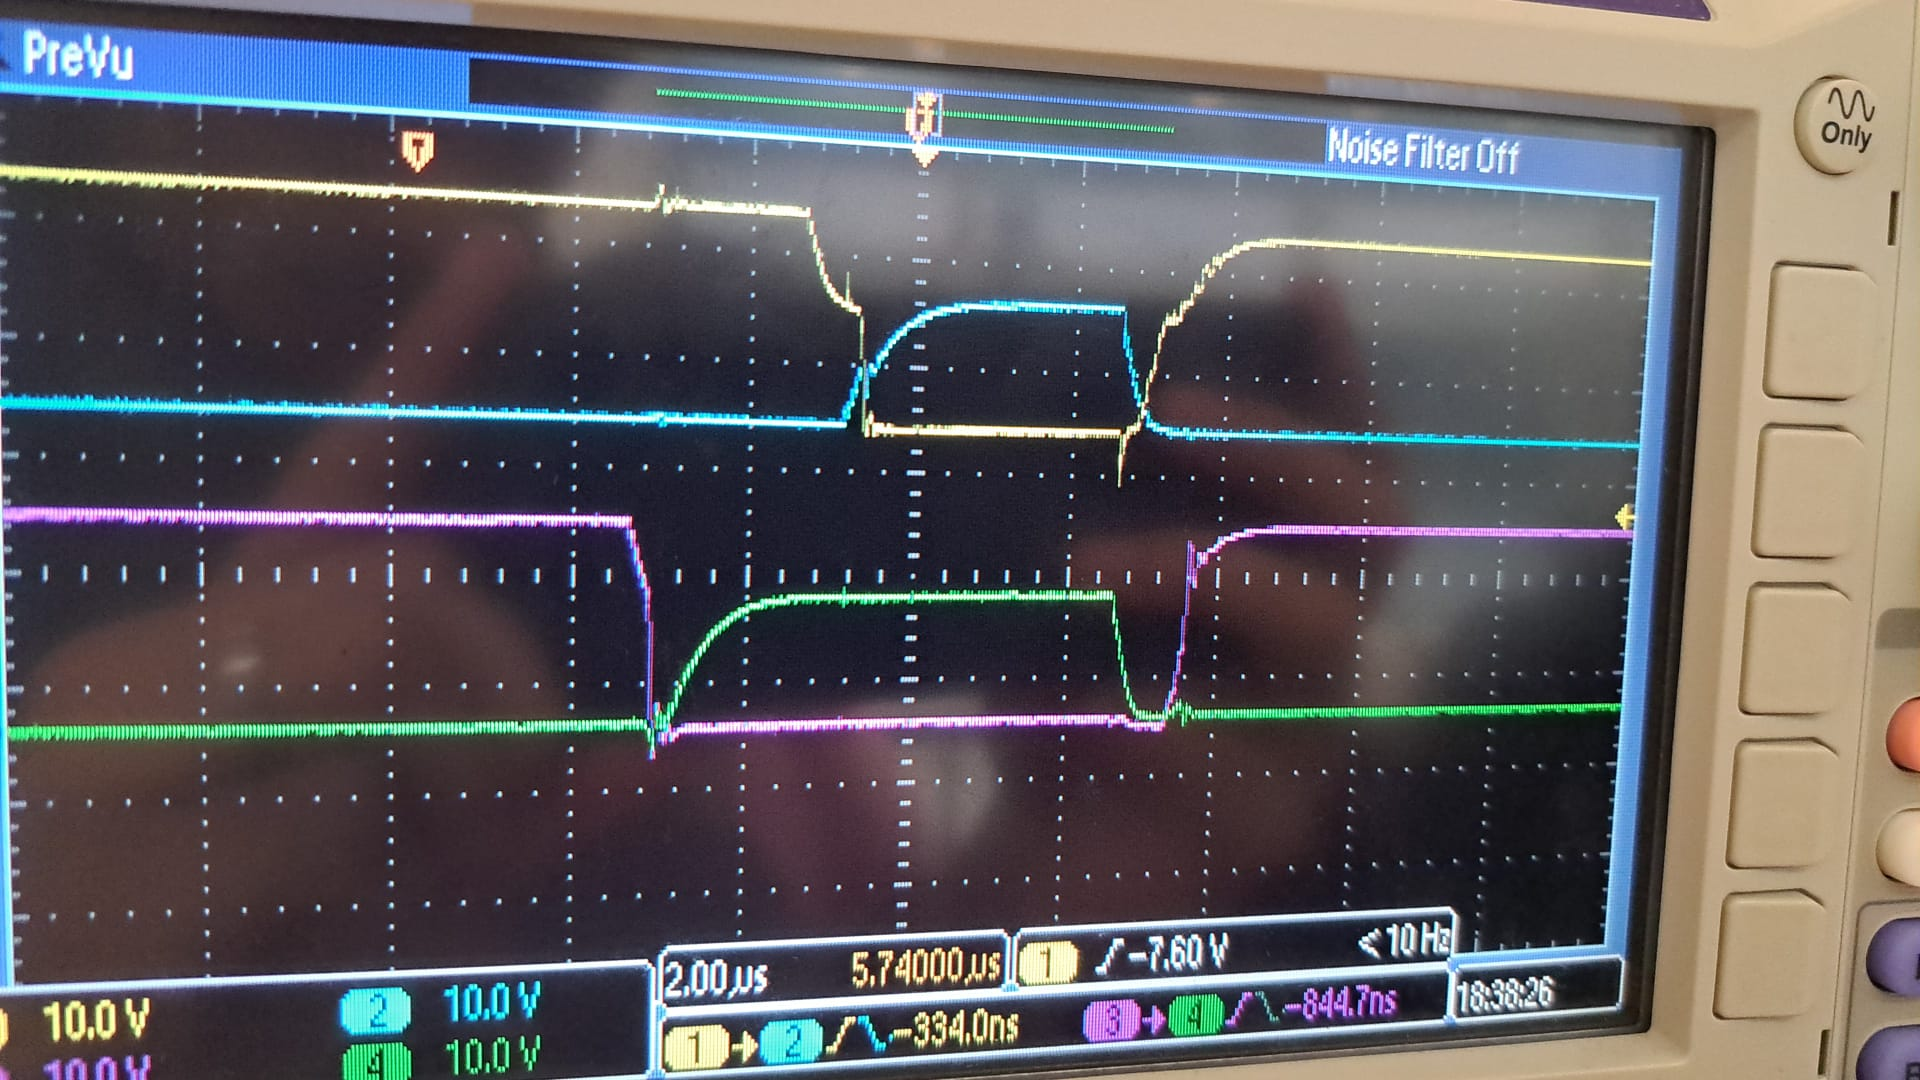
\includegraphics[width=\linewidth]{img//GateDriver/WhatsApp Image 2024-03-18 at 18.38.31_9fd81adb.jpg}
        \caption{Boven 5 ohm, onder 1 ohm.}
         \label{fig:smallshort}
    \end{subfigure}
    \hfill
    \begin{subfigure}{0.32\textwidth}
    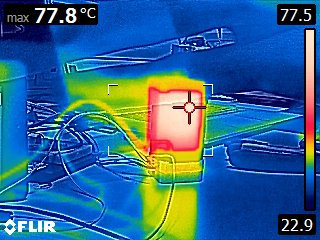
\includegraphics[width=\linewidth]{img/WhatsApp Image 2024-03-28 at 18.31.53_bad388f9.jpg}
    \caption{Enter Caption}
    \label{fig:BLDCHEAT}
    \end{subfigure}
    \hfill
  \label{fig:Buck}
  \caption{Testing}
\end{figure}


\subsection{MOSFET}\label{MOSFET}
The MOSFETs selected for the circuit are the IPP015N04NF2S\cite{infineon-ipp015n04nf2s-datasheet}. These MOSFETs work flawless within our circuit, requiring minimal testing. With a voltage rating of 40V and a current rating of 193A, they are well-suited to operate effectively within our 24V system.

\subsection{Buck Converter}\label{Buck converter}
The buck converters were designed with WeBench, following a recommendation from Diego. Two buck converters were created with the TPS62932\cite{ti-tps62932-datasheet} IC: one to step down 24V to 12V for the gate driver and another to step down 24V to 5V for the STM32F411\cite{stm32-base-board}, user interface, and Hall sensors. Extensive simulations and testing were conducted, confirming the effectiveness of the design. Upon subjecting the buck converters to a load (refer to \autoref{fig:BuckLoad}) of \(\frac{3\times50\Omega}{150\Omega}=16\frac{2}{3}\Omega\), both simulation and test results exhibited close correlation. Additionally, temperature readings (refer to \autoref{fig:BuckTemp}) revealed that the buck converter under this high load condition could reach elevated temperatures over prolonged periods of operation. An heatsink might be smart in the future.
\begin{figure}[H]
    \centering
    \hfill
    \begin{subfigure}{0.23\textwidth}
        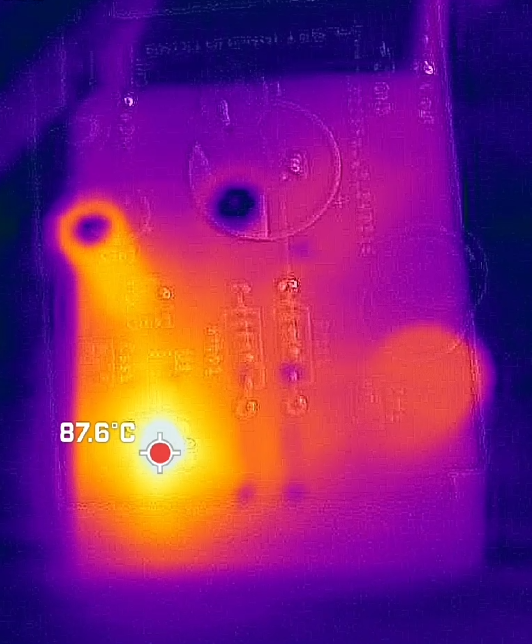
\includegraphics[width=\linewidth]{afbeelding2.png}
        \caption{Temp reading: Buck converter IC after 10min with load}
        \label{fig:BuckTemp}
    \end{subfigure}
    \hfill
    \begin{subfigure}{0.3\textwidth}
        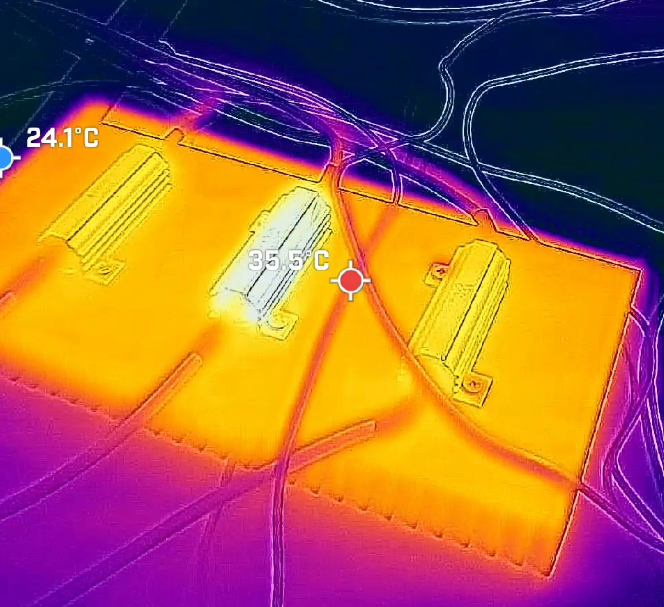
\includegraphics[width=\linewidth]{afbeelding.png}
    \caption{Temp reading: Buck converter load \(16\frac{2}{3}\Omega\).}
    \label{fig:BuckLoad}
    \end{subfigure}
    \hfill
  \label{fig:Buck}
  \caption{Buck converter testing}
\end{figure}



\subsection{BLDC}\label{BLDC}
Following thorough testing, it was observed that the hall sensors were not transmitting data as desired. Subsequently, a different motor was employed, yielding improved results. The feedback loop from our code to the gate drivers behaved as anticipated. Initially, it was not suspected that the motor itself was faulty. The defective BLDC motor\cite{reichelt-motor-datasheet} was entrusted to Stephen for further analysis, and a replacement motor was obtained, which functioned flawlessly.
\subsubsection{Temperature}
We have done some extensive testing into current drawnings. We have set the BLDC motor\cite{reichelt-motor-datasheet} under a load to see what would happend. We concluded that as the datasheet has given we motor indeed doens't have a lot of torque. Also we have done a lot of temperature measurements which resulted us in us changing code/hardware. We realized we were getting a short as told in \autoref{Gate driver}

\subsection{Interface}\label{Interface}
A decision was made to utilize a Raspberry Pi\cite{raspberrypi-3b} as the front-end interface\cite{sossolutions-7inch-touchscreen}. Establishing a rapid communication method was a priority, leading to the adoption of the I\textsuperscript{2}C protocol. Encounter of issues arose when the STM32F411\cite{stm32-base-board} struggled to receive the data, prompting the connection of pins to an oscilloscope to verify signal transmission. Upon confirmation that the issue was software-related, appropriate adjustments were made to resolve it.

\subsubsection{Current sensing}\label{Current Sensing}
In response to the project lead's requirement, we selected the INA181A3QDBVRQ1\cite{ti-ina181-q1} for current sensing, utilizing it alongside a shunt resistor to measure BLDC motor\cite{reichelt-motor-datasheet} current. This automotive-grade amplifier converts current to voltage for the STM32\cite{stm32-base-board} ADC to read. However, we recognized the potential for improvement and decided to explore the INA236BIDDFR\cite{ti-ina236-datasheet}, offering a 16-bit ADC interface via I\textsuperscript{2}C, providing significantly higher resolution than the STM32F411's\cite{stm32-base-board} 12-bit ADC. This upgrade promises enhanced accuracy with \(2^{16}-2^{12}=61440\) additional data points, although testing of this configuration is pending.